\section{Download files}
{Once a project is created, the first step is to download the files from the different websites in order to have the data available.}
\begin{figure}[H]
\centering
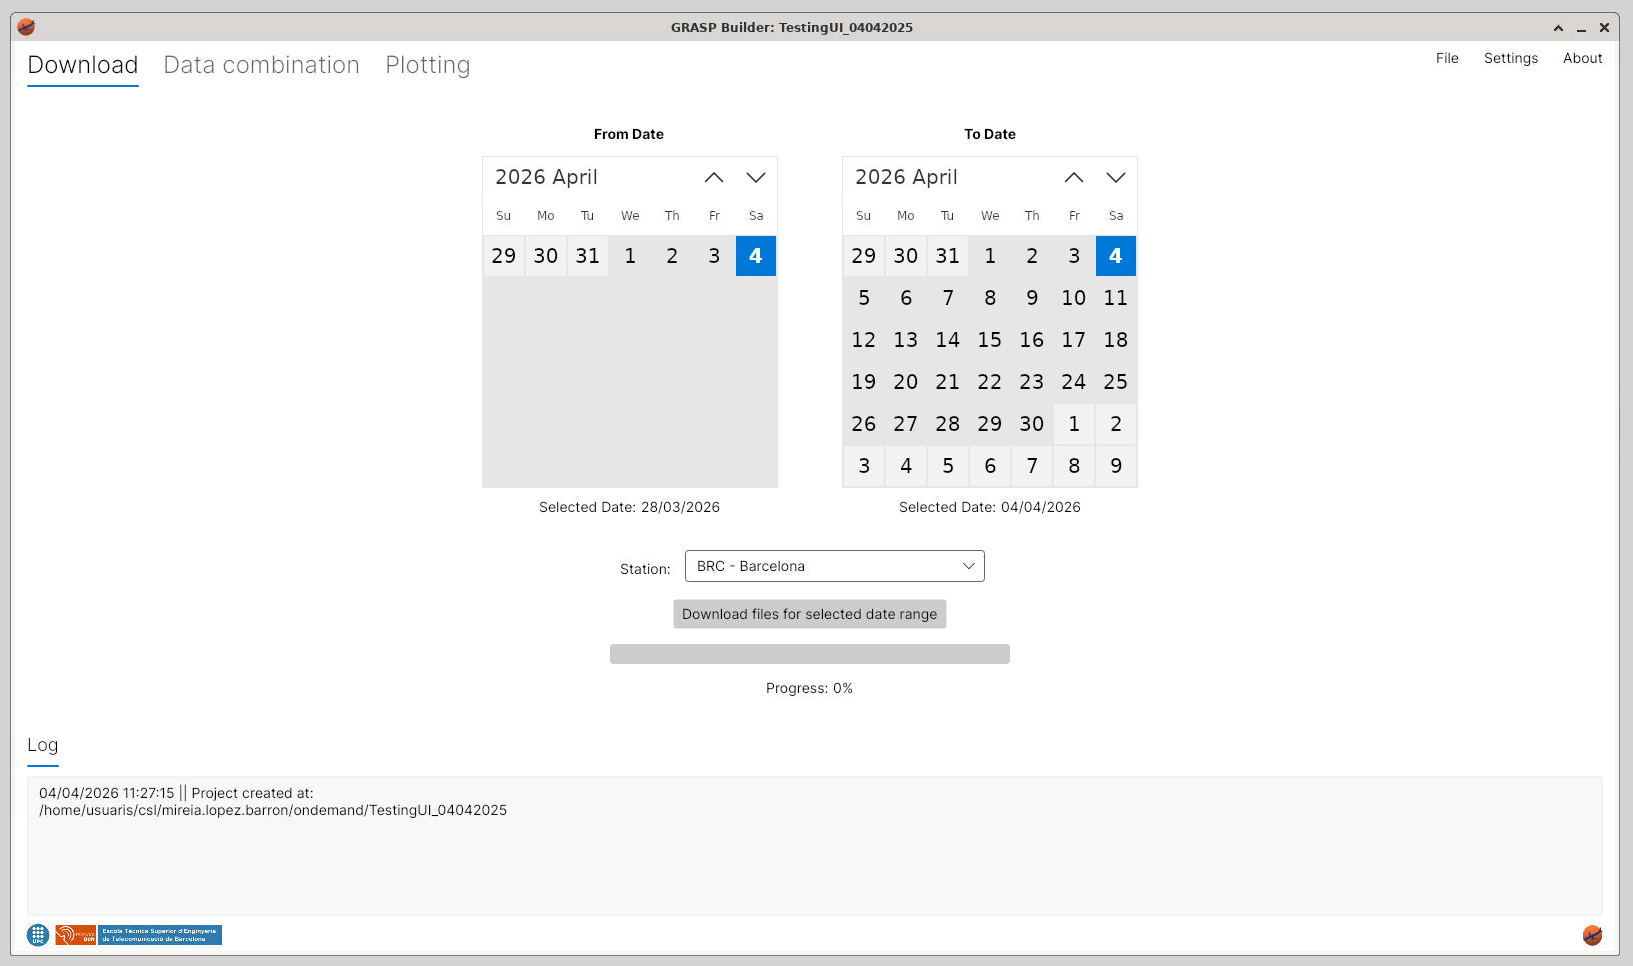
\includegraphics[width=16cm]{img/ProjectLoaded_noFiles.png}
\caption[Project loaded]{\footnotesize{Project loaded}}
\label{fig:ProjectOpenedDownload_noFiles}
\end{figure}


{In this tab, the user is available to choose the range of dates to download the files from the different websites. For the moment, it is only available to download files from the selected site. Available sites are locations that have data in both websites, Aeronet and Earlinet. Sites that only have data in one of them are descarted, since it is necessary files from both platforms in order to run the GRASP algorithm.\smallskip\\
During the process, all buttons will be disabled and the progress bar will show the percentage of files downloaded. Once all files are downloaded, a new section will be shown where the user will be able to see the list of files downloaded and select the files that desires to keep. This section will be also shown if the user opens a project with already downloaded files (\Cref{fig:ProjectOpenedDownload}). }

\begin{figure}[H]
\centering
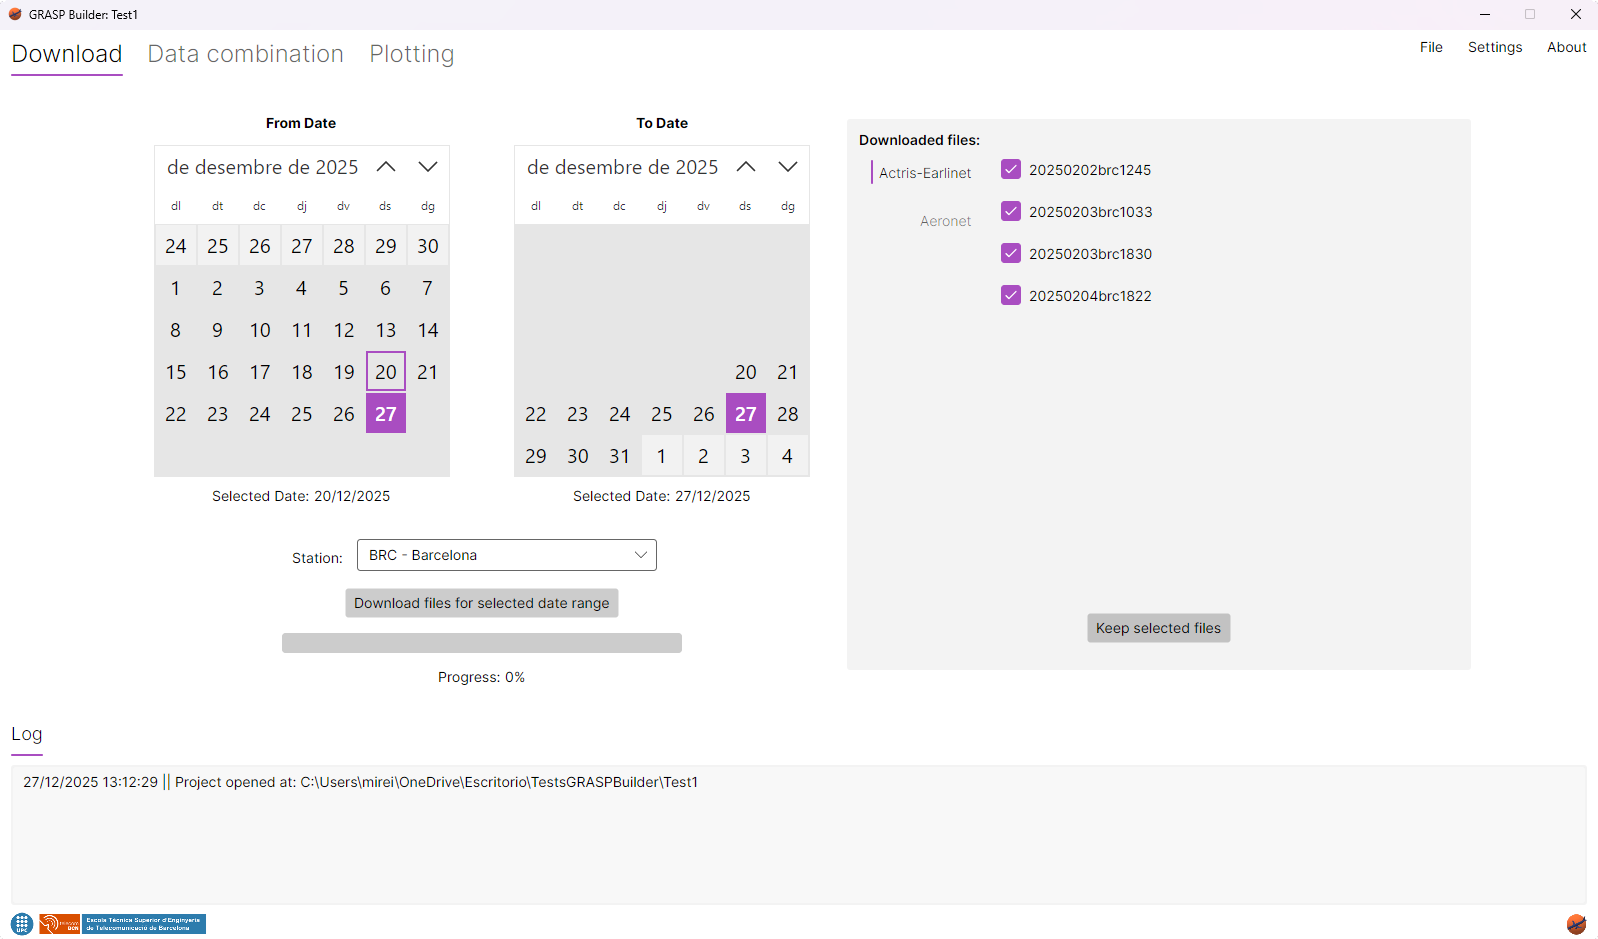
\includegraphics[width=16cm]{img/ProjectOpenedDownload.png}
\caption[Project loaded]{\footnotesize{Files downloaded}}
\label{fig:ProjectOpenedDownload}
\end{figure}
